\section{Computational Steering Using Sparse Grids}
\label{sec:comp_steering}

Our application is the visualization of compressed, high-dimensional data
resulting from simulations \cite{Butnaru201156}. It is well known that managing
data coming from high-dimensional functions has an exponential complexity on the
number of dimensions. Therefore, we compress the data using the sparse grid
technique in order to reduce its size and decompress it afterwards for real-time
visualization. For this purpose we use the \textit{fastsg}
library~\cite{murarasu12fastsg:}.

The main idea behind sparse grids is that we can approximate a $D$-dimensional
function $f : \Omega \rightarrow \mathbb{R}$, where $\Omega = [0, 1]^{D}$, by
discretizing $\Omega$ and representing $f$ as a weighted sum of \textit{basis
functions}. If we consider \textit{levels} $\bar{l} = (l_{1},\ldots,l_{D})$ and
\textit{index} $\bar{i} = (i_{1},\ldots,i_{D})$ vectors in $\mathbb{N}^{D}$,
then each basis function will be centered at points $\bar{x}_{\bar{l},\bar{i}} =
(x_{l_{1},i_{1}},\ldots,x_{l_{D},i_{D}}) \in \mathbb{Q}^{D}$, for which $x_{l,i}
= i \cdot 2^{-l}$, $i \in \{1,\ldots,2^{l} - 1\}$, and $i$ odd. This means that
each grid point $\bar{x}_{\bar{l},\bar{i}}$ can be uniquely identified by the
pair $(\bar{l},\bar{i})$. Thus,

\[ f \approx \sum_{\bar{x}_{\bar{l},\bar{i}}} \alpha_{\bar{l},\bar{i}} \cdot
\phi_{\bar{l},\bar{i}} \]
where $\alpha_{\bar{l},\bar{i}}$ is the weight, or \textit{hierarchical
coefficient}, and $\phi_{\bar{l},\bar{i}}$ is the basis function centered at
grid point $\bar{x}_{\bar{l},\bar{i}}$. In our case, $\phi_{\bar{l},\bar{i}}$ is
obtained by multiplying $D$ one-dimensional functions $\phi_{l,i} = h(2^{l}x -
i)$, where $h$ is the standard hat function $h(x) = max(1 - |x|, 0)$:

\[ \phi_{\bar{l},\bar{i}}(\bar{x}) = \prod_{t=1}^{D} \phi_{l,i}(x_{t}) .\]

The \textit{truncated sparse grid}, $\Omega_a \subseteq \Omega_r$, identified by
a given constraint vector $\underline{c}$, is the set of points
\begin{equation*}
\Omega_a := \{\bar{x}_{\bar{l}, \bar{i}} : |\bar{l}|_1 \leq L
+ D - 1, l_t \leq c_t,  t \in \{1, \dots, D\}\}.
\end{equation*}
If $c_t = L, \forall 1 \leq t \leq D$ then $\Omega_a$ becomes a regular sparse
grid, i.e. regular sparse grids are special types of dimensionally truncated
sparse grids.


Compressing a general function represented on a full grid is done by selecting
only the function values at grid points also contained in the sparse grid $\Omega_a$. 
Many points are excluded from the full grid using the $\Omega_a$ discretization,
thus resulting in a form of lossy compression. 
Sparse grids theory is based on the fact that the excluded points have a reduced
contribution to the approximation \cite{CambridgeJournals:227245}. The
consequence is that for sufficiently smooth functions, removing the points does
not significantly deteriorate the accuracy compared to full grids.
Compression is reduced to computing the hierarchical coefficients $\alpha$,
process called \textit{hierarchization}. Decompression, also called
\textit{evaluation} or \textit{interpolation}, refers to evaluating the sparse
grid approximation anywhere inside the domain by summing up the contributions of
the basis functions averaged by their hierarchical coefficients. This also
enables us to interpolate at points for which we do not have values from
simulation. Hence, it can provide hints on the simulation outside the initial
data. In our case, decompression is based on the sparse grid technique described
in \cite{CambridgeJournals:227245}.

\begin{figure}[t]
  \begin{subfigure}[b]{1\linewidth}
    \centering
    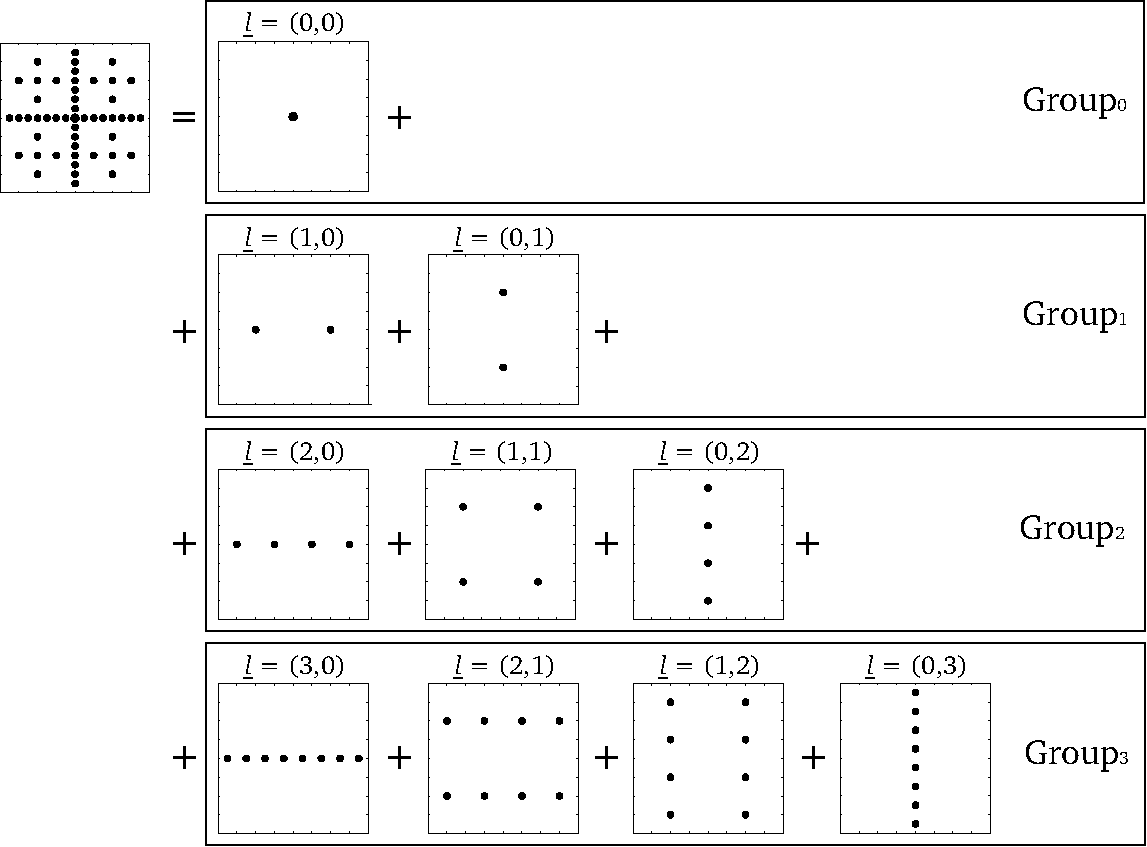
\includegraphics[width=0.9\textwidth]{truncated_sparse_grid_deco_1.pdf}
    \caption{Regular sparse grid.}
    \label{fig:truncated_sparse_grid_deco_1}
  \end{subfigure}
  \\ \\
  \begin{subfigure}[b]{1\linewidth}
    \centering
    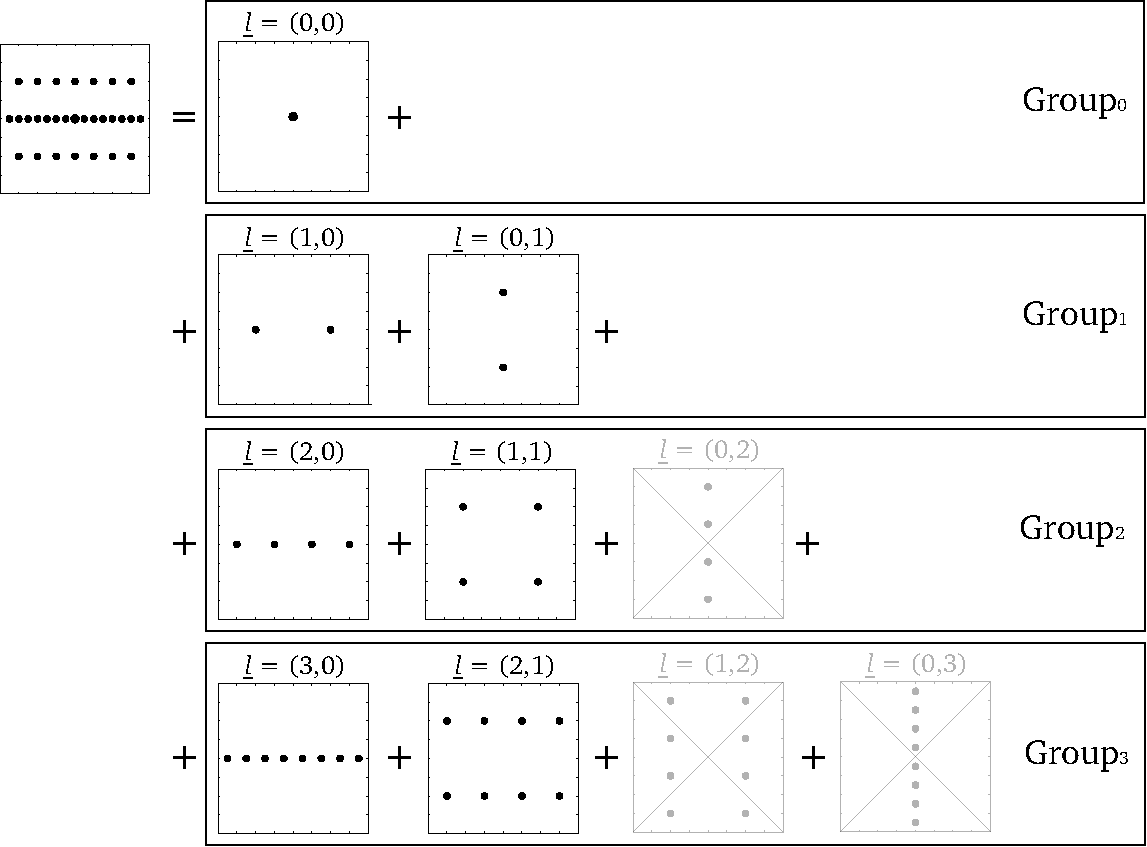
\includegraphics[width=0.9\textwidth]{truncated_sparse_grid_deco_2.pdf}
    \caption{Dimensionally truncated sparse grid.}
    \label{fig:truncated_sparse_grid_deco_2}
  \end{subfigure}
  \caption{Decomposition of 2D sparse grids.}
  \label{fig:truncated_sparse_grid_deco}
\end{figure}

\subsection{Compression}

It is important that sparse grids should not be confused with sparse matrices.
They differ in both functionality and computational behavior. As mentioned,
sparse grids allow us to approximate multi-dimensional functions. The method is
somehow related to wavelet transformation technique \cite{Mallat89atheory},
where computing and grouping of the coefficients leads to a multi-scale
representation. Similar to wavelet compression, we also have here a hierarchical
representation which corresponds to different scales or levels of detail. The
contribution of the coefficients reduces as this level increases.

Sparse grid compression has 4 input parameters: number of dimensions $D$,
refinement level $L$, precision $P$ (single or double precision), and truncation
$T$ (dimensionally truncated or regular). $T$ gives the possibility of reducing
the computational effort when using functions where not all dimensions carry
equal weight. Therefore, instead of storing all regular grids, we can exclude
some of them when the information on those dimensions is not critical (see Fig.
\ref{fig:truncated_sparse_grid_deco_2}). In our case, this translates to
restricting the components of the $\bar{l}$ vector. An analogy can be made with
image compression. Usually images are not squares, but rectangular in shape,
having the width twice the size of their height. Going back to our sparse grids
domain, we can thus use a refinement level in one dimension (width) equal to 2x
the refinement level in the other dimension (height).

Fig.~\ref{fig:truncated_sparse_grid_deco_1} shows how a sparse grid can be
represented as a sequence of regular grids, grouped by their norm into several
refinement levels, which will be simply referred to as \textit{groups}. The
grids in one \textit{group} will be called \textit{blocks}\footnote{Grid
\textit{blocks} should not be confused with CUDA thread \textit{blocks}.}.
Instead of using the traditional approach of storing the grids in trees and
hash-tables, we are using a bijection based data structure with minimum memory
footprint \cite{Murarasu:2011:CDS:1941553.1941559}. All hierarchical
coefficients are efficiently stored in a 1-dimensional array, by mapping
$(\bar{l},\bar{i})$ pairs to consecutive integer indices.

Compressing the multi-dimensional function translates to computing the
hierarchical coefficients, in a traditionally recursive manner by collecting the
contributions of all points and evaluating the basis functions in each
dimension. With the above data structure, we can use a non-recursive
GPU-friendly algorithm for compression. Although this algorithm is
integer-bound, the next section shows that it can be made memory-bound by
applying different loop transformation.

\subsection{Decompression}

Interpolating at a given $D$-dimensional point means traversing the set of
regular grids and computing the contribution of each one. For each regular grid,
a $D$-linear basis function is built in $\mathcal{O}(D)$ and evaluated at that
point. Interpolating at one point uses exactly one value from each regular grid
for scaling the basis function. We can now analyse the influence of input
parameters on the performance of interpolation, visible especially on GPUs.

Sparse grid decompression has 5 input parameters: number of dimensions $D$,
refinement level $L$, number of interpolation points $N$, precision $P$, and
truncation $T$. $D$ increases the computational intensity, i.e. the ratio
between the on-chip computation time and off-chip communication time. On GPU, a
large $D$ causes an increased consumption of shared memory per thread reducing
the benefits of multithreading. A large $L$ decreases the computational
intensity since the size of the regular grids increases exponentially, i.e. from
$2^0$ to $2^{L-1}$.
